\subsection{Normalización}

\subsubsection{Funcionamiento de los Contratos}

\qquad Existe un problema al querer analizar los datos de los valores observados de los contratos, y es que no todos funcionan de la misma manera. Esto es una complicación ya que significa que los datos de la matriz no representan lo mismo con respecto al largo del intervalo de su contrato, haciendo que no sean comparables.

\qquad Las tasas de interés de los contratos de 1 a 18 meses se les dice cero cupón. Esto se debe a que desde el inicio del contrato, solo se hace el intercambio de flujo al finalizar el periodo de tiempo, lo que es el pago del nominal mas los intereses correspondientes.
\begin{figure}[H]
  \centering
      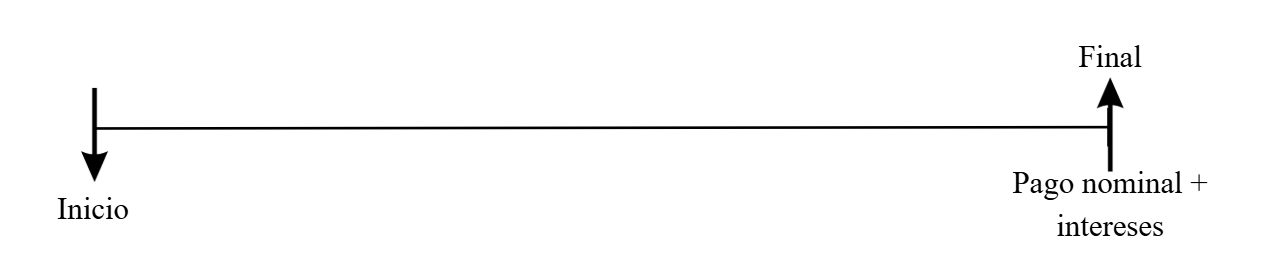
\includegraphics[scale=0.45]{images/diagrama_contratos_cero_cupon.png}
  \caption{Diagrama contratos cero cupón
  }\label{fig:0cupon}
\end{figure}

\qquad Por otro lado, los contratos de 2 a 25 años funcionan con cupones semestrales, es decir, cada seis meses desde el inicio del contrato se hace un depósito de intereses.
\begin{figure}[H]
  \centering
    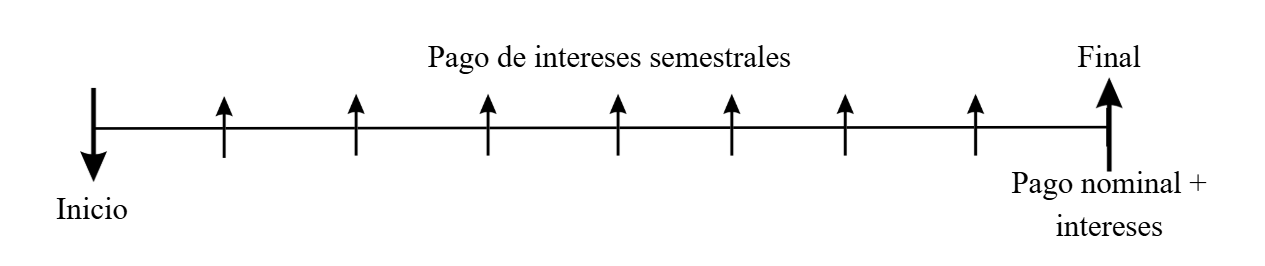
\includegraphics[scale=0.45]{images/diagrama_contratos_semestrales.png}
  \caption{Diagrama contratos con cupones semestrales
  }\label{fig:0cupon}
\end{figure}

\subsubsection{\textit{Bootstrapping}}

\qquad Para solucionar este problema existe un proceso llamado \textit{Bootsraping} financiero. El cual consiste en construir una curva de tasas de cero cupón a partir de los precios de un conjunto de productos con cupones. En otras palabras, para cada contrato que funciona con cupones, queremos encontrar una tasa cero cupón equivalente.

\qquad Para esto utilizamos el factor de descuento, el cual se define de la siguiente manera
$$ \text{DF}(0,T) := \text{El precio hoy de recibir una unidad de dinero en el tiempo } T.$$
Notar que este valor es universal y no depende de los contratos. Sin embargo, es posible saber su valor a través de las tasas de interés de los contratos swap. Para un contrato swap cero cupón a un plazo $T$ y valor $r_T$, el factor de descuento se calcula de la siguiente manera
\begin{equation}
    \text{DF}(0,T) = \dfrac{1}{1 + r_T \frac{\text{buss}(T)}{360}},
\end{equation}
donde $\text{buss}(T)$ es la cantidad de días hábiles en el periodo $T$. Por otro lado, si es que el contrato funcionará con cupones semestrales, el factor de descuento se calcularía así
\begin{equation}
    \text{DF}(0,T) = \dfrac{1 - \sum_{i= 6\text{M}}^{T - 6\text{M}} \frac{\text{buss}(\Delta T_i)}{360} \text{DF}(0, T_i)}{1 + r_T \frac{\text{buss}(\Delta T)}{360}},
\end{equation}
donde $\text{buss}(\Delta T_i)$ corresponde a los días hábiles en tal periodo de 6 meses. Teniendo el factor de descuento, se puede utilizar la ecuación (1) para despejar la tasa cero cupón equivalente, obteniendo así

\begin{equation}
    r_T^{\text{0cupón}} = \dfrac{360}{\text{buss}(T)}\left( \dfrac{1}{\text{DF}(0,T) - 1}\right).
\end{equation}

\qquad Sin embargo, existe un problema. Notar que en la ecuación (2) se es necesario el valor de $\text{DF}(T_i)$ para cada semestre entre el inicio y el final del contrato. Conocer este valor de manera directa no es posible ya que hay $T_i$'s, por ejemplo 30 meses, en los que no existe contrato, por ende no existe una tasa con la cual calcular tal factor de descuento.

\qquad Existen varias formas de resolver este problema, para efectos de esta etapa exploratoria de los datos decidimos realizar una interpolación lineal para la tasa de cada $T_i$ necesario. Por ejemplo, la tasa ficticia para un contrato de 30 meses, con cupones semestrales, se calcula como el promedio entre la tasa de los dos años y tres años.

$$r_{30 \text{M}} = \dfrac{r_{2 \text{Y}} + r_{3 \text{Y}}}{2}.$$

\begin{figure}[H]
    \centering
        \includegraphics[scale=0.45]{images/seriestemporales0cupon.png}
    \caption{Curva de tasas cero cupón
    }\label{fig:0cupon}
\end{figure}
\subsection{PCA}
\qquad Una vez que todos los contratos están normalizados a tasas cero cupón, 
es posible 
comparar los datos entre sí. Sin embargo, sigue existiendo el problema de la 
dimensionalidad. En este caso, cada observación tiene 17 dimensiones, lo que 
hace difícil 
analizar los datos y encontrar patrones. El modelo que utilizaremos recibe 
como input una 
tasa, es por ello que caracterizar los datos en una sola dimensión es 
crucial. 

Litterman y Scheinkman (1991) observaron que con 3 componentes es posible describir el 99\% de la variabilidad observada en el mercado, en particular, la primera componente explica aproximadamente el 96\% de la variabilidad \cite{pca}.

Al realizar PCA obtuvimos que las primeras 2 componentes explican el 98\% de la varianza, pero la primera componente solo explica el 81.5\% de la variabilidad. Este resultado es bajo respecto a lo esperado, pero puede ser explicado por el corto periodo que abarcan los datos, de 2021 a 2025 y por el contexto económico particular de este periodo, que incluye a la pandemia y una alta inflación. 
\begin{figure}[H]
    \centering
        \includegraphics[scale=0.7]{images/pca.png}
    \caption{Varianza explicada por cada componente principal
    }\label{fig:varpca}
\end{figure}
\subsection{La tasa corta}
\qquad A pesar de que la primera componente no explicó de forma esperada la variabilidad de la muestra, podemos interpretar esta componente como la tasa corta (1M), pues esto se debe a fenómenos relacionados al contexto de la muestra y que al variar el nivel de la tasa corta, esta sigue controlando y captura de buena manera el comportamiento de los 17 tenores. En el siguiente gráfico podemos observar la correlación entre la tasa corta (1M) junto a la TPM, notando como la tasa corta sigue de buena manera el comportamiento de la TPM.
\begin{figure}[H]
    \centering
        \includegraphics[scale=0.45]{images/tasacortatpm.png}
    \caption{Tasa corta (1M) vs TPM
    }\label{fig:varpca}
\end{figure}
Por la naturaleza de la TPM, el mercado busca anticiparse a los cambios de la TPM, esto provoca ese efecto “serrucho”, donde la tasa corta (1M) sube antes que la TPM y baja después de la TPM. 

Dado que la tasa corta (1M) explica gran parte de la variabilidad 
de los datos y que tiene sentido económico, se decidió utilizar 
esta tasa para calibrar el modelo.